\part{Exploration du corpus Indochine}

\chapter{Un corpus scientifique important de l'Indochine}

\section{Base de données}

\subsection{Collection des Bulletins de la Société des études Indochinoises}

Le Bulletin de la Société des Études Indochinoises est une publication spécifiquement sélectionnée pour être numérisée dans le cadre du projet VALEASE (Valorisation de l'écrit en Asie du Sud-Est) depuis 2005. Ce projet consiste en une base de données numérique totale qui compte 540.000 pages de texte, soit 5\% des ressources de la Bibliothèque scientifique générale de Hô Chi Minh-Ville. Ce projet fait partie de la Bibliotheca Vietnamica, qui vise à numériser les archives de documents français anciens considérés comme un patrimoine national du Vietnam. L'objectif est de diffuser largement ces documents en Asie du Sud-Est et dans le monde entier. Parmi ces documents, on trouve de nombreuses publications rares des XVIe, XVIIe et XVIIIe siècles, telles que \textit{DelFhistoria della China} (1586), \textit{Dictionarivm annamiticvm lvsitanvm}, et \textit{latinvm ope sacrae congregations de propaganda fide in lvcem editvm AB / Alexandre de Rhodes} (1651), \textit{Voyage du Siam} (1666), \textit{Le grand dictionnaire historique, ou le mélange curieux de l'histoire sacrée et profane de Louis Moréri} (1759), et \textit{Voyage au Tonkin} (1788).

Les revues scientifiques numérisées dans le cadre du projet comprennent: Bulletin des Amis du Vieux Huê (BAVH) (1914-1923), Bulletin de l'École française d'Extrême-Orient (BEFEO) depuis 1901 , la revue Sudia (Van Su Dia) (1969-1975), ect.

Ces sources documentaires sont disponibles, pourtant elles manquent de recherches ultérieures approfondies sur le contenu des documents ainsi que sur les systèmes organisationnels qui les sous-tendent, sur les sujets, les auteurs, les fonctions, la quantité de journaux, les méthodes d'organisation et les institutions financières. Toutes ces informations, issues de documents authentiques, sont utiles pour mieux comprendre l’histoire de l’Indochine.

La qualité des fichiers PDF varie de 300 DPI, ce qui comprend les numéros annuels, soit un total de 82 dossiers avec 164 numéros. Les données des numéros de journaux ont ensuite été compilées manuellement par l'équipe Vietnamica sous la forme d'un fichier Excel qui contient les titres d'articles en français, traduits en deux langues (anglais et vietnamien), les numéros de journaux et les numéros de pages (sur le PDF et les pages sur papier). Les articles sont également divisés en 14 sections, dont la section "Autres" comprend la majorité des numéros divers non catégorisés. Le processus de classification étant effectué manuellement, l'équipe sélectionne uniquement les éléments clairement mentionnés et ne se penche pas sur les genres d'articles scientifiques. Ces paramètres sont nécessaires pour l'étape suivante du traitement, qui consiste à découper les numéros des journaux en fonction des articles. Cette étape est réalisée à l'aide de scripts PHP sur la page source de la bibliothèque électronique et les articles sont regroupés en sections, notamment : 

\begin{itemize}
    \item 15 unités Actes De La Société
    \item 35 unités bibliographies
    \item 10 unités Sociétés Correspondantes
    \item 15 unités Bureau De La Société Des Études Indochinoises
    \item 6 unités catalogues
    \item 12 unités Communications, Congrès et Allocutions
    \item 141 unités Etudes, Notes et Avis
    \item 35 unités Liste des Membres et Assemblées générales
    \item 12 unités Nécrologies
    \item 98 unités Procès-Verbaux
    \item 42 unités publications
    \item 34 unités Rapports et Comptes-rendus
    \item 18 unités Statuts De La Société Des Études Indochinoises
    \item 774 unités Autres
\end{itemize}

Les articles sont ensuite téléchargés dans la bibliothèque numérique du projet Vietnamica à l'adresse : https://revues.vietnamica.online/version2/bsei/

L'état actuel des données pour la réalisation de ce mémoire est que les numéros du bulletin ont été préalablement découpés. Pour passer à l'étape suivante, qui consiste à former un modèle textuel spécifique au corpus via le logiciel Kraken, nous avons sélectionné une liste d'articles pour la transcription manuelle, servant d'échantillons pour le modèle. Dans le but de mettre en œuvre un modèle mixte adapté au corpus, nous avons choisi les critères suivants :

\begin{itemize}
    \item Articles courts, mettant l'accent sur le contenu important (en fonction du titre de l'article).
    \item Des articles provenant de différentes étapes (afin de diversifier les échantillons d'écriture).
    \item Articles multilingues ou purement vietnamiens.
    \item Les fichiers utilisés pour la formation ont été téléchargés directement sur eScriptorium, reconnus par le modèle français automatique du site, puis corrigés manuellement. 

Les annotations ont ensuite été exportées vers le fichier ALTO et ont servi lors de 5 sessions de formation au total :
\end{itemize}

\begin{itemize}
    \item 700 pages de textes en français du B.S.E.I
    \item 400 pages de textes quoc ngu-français du B.S.E.I
    \item 500 pages de quoc ngu d'autres souces
\end{itemize}

\begin{figure}
    \centering
    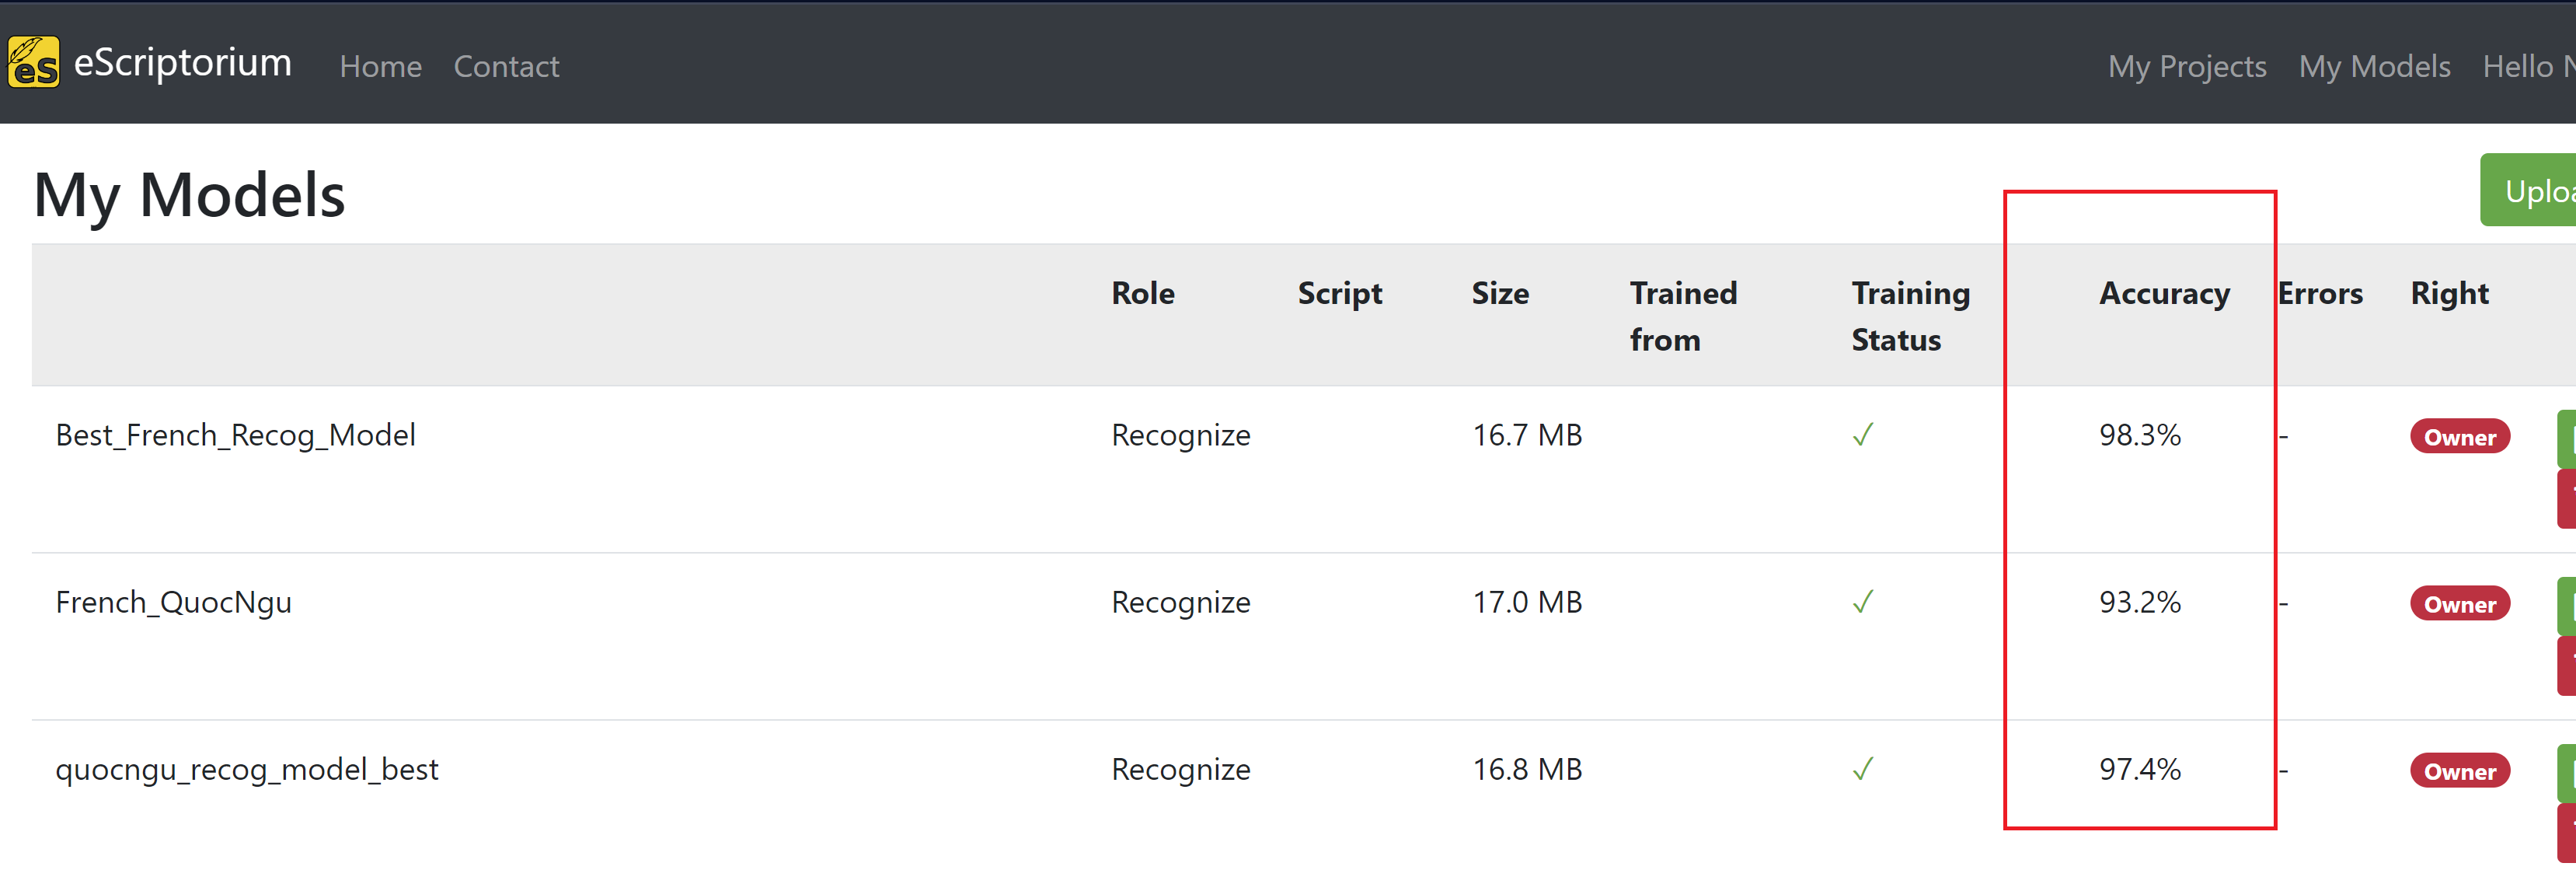
\includegraphics[width=1\linewidth]{img/model3.PNG}
    \caption{Les trois modèles principaux}
    \label{fig:enter-label}
\end{figure}

\textbf{Résultat :} 

\begin{enumerate}
    \item un modèle mixte atteint 93,2\% d'efficacité
    \item un modèle quoc-ngu 97\% d'efficacité
    \item Un modèle français 98.3\% d'efficacité
\end{enumerate}

Nous utilisons le modèle mixte pour exploiter le corpus B.S.E.I dans le cadre de ce projet. Cependant, ce modèle n'est réellement efficace qu'avec le français, et les parties vietnamiennes sont pratiquement inutilisables pour notre exploitation. Cela est en partie dû au faible nombre de textes en vietnamien dans le corpus, ce qui se reflète dans le processus de sélection manuelle des échantillons pour la formation. Avec un corpus comme le B.S.E.I, un modèle ayant une efficacité de 93,2\% est acceptable pour les premières expériences de recherche.

Le corpus du Bulletin de la Société des Études Indochinoises (B.S.E.I) revêt une importance capitale au sein de la bibliothèque numérique Vietnamica. Cette source regroupe un total de 1 342 articles numérisés, tâche entreprise par l'équipe du projet européen Vietnamica, centré sur la recherche historique et la numérisation de documents épitaphes vietnamiens.

De plus, 26 numéros du B.S.E.I sont également consultables dans la bibliothèque Galica, avec leur modèle français atteignant un taux d'efficacité de 87,95\%. À l'heure actuelle, l'intégralité des numéros du Bulletin de la Société des Études Indochinoises est accessible en libre consultation via l'adresse numérique du projet.

Les documents utilisés dans cette étude sont des numéros du B.S.E.I numérisés au format PDF. Le Bulletin a été publié pour la première fois à Saigon en 1883, succédant ainsi au Bulletin du Comité Agricole et Industriel de la Cochinchine (1865-1882). Selon les informations fournies dans le dernier numéro du B.S.E.I datant de 1975, il est possible de distinguer deux étapes cruciales dans le développement de cette publication :

\begin{itemize}
    \item 1883-1823 Ancienne série volumes 1-71 appelée Bulletin de Saigon
    \item  1826-1975 Nouvelle série change son nom pour Bulletin
\end{itemize}
Il convient de noter qu'il manque un numéro daté de 1938 dans le corpus, en raison de contraintes liées à la collecte des données.
\begin{figure}
    \centering
    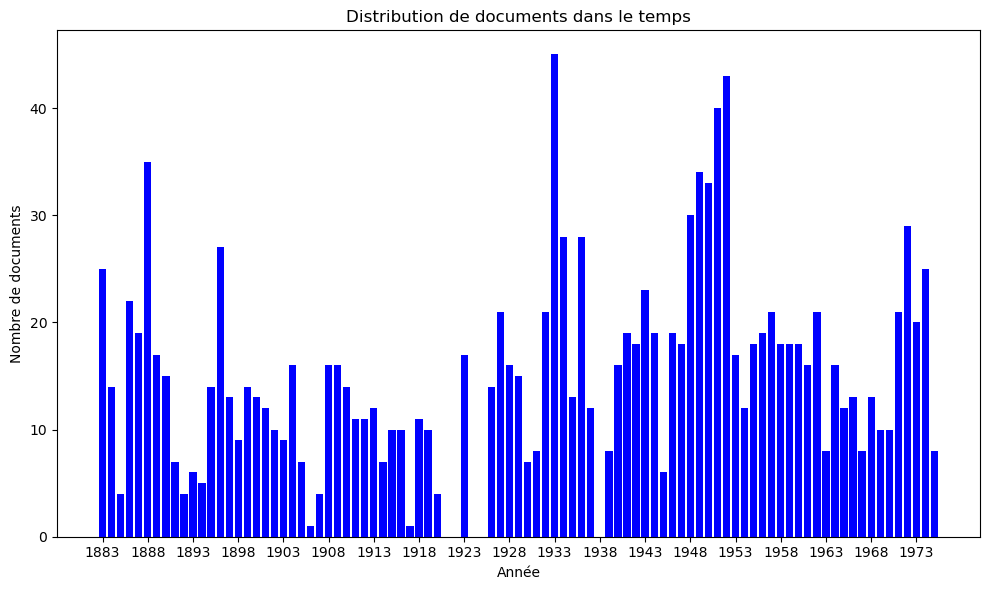
\includegraphics[width=1\linewidth]{img/2.1.nb_doc_year.png}
    \caption{Distribution de documents dans le temps}
    \label{fig:nb_doc_year}
\end{figure}

Parmi ces éditions, il y avait une réédition des volumes de l'édition originale datant de 1974, et ces publications étaient disponibles à la vente dans les bibliothèques correspondantes à Saigon, Hong Kong, Paris, et Bruxelles.

Parmi les volumes du B.S.E.I, deux publications d'une importance particulière ont été extraites et ultérieurement publiées de manière indépendante : 
\begin{itemize}
    \item Les Bas-Reliefs des Urnes Dynastiques de Hue par le R.P Bar-Nouin (1974)
    \item Historique romain des Trois Royaumes (trad. Nghiem Toan et Louis Ricaud) (1960-1963)  
\end{itemize}

Parmi eux, le Roman Historique des Trois Royaumes est réédité chez Flammarion depuis 2009 en France. \footnote{https://editions.flammarion.com/les-trois-royaumes-1/9782081225541}

Pour cette étude, notre attention sera exclusivement portée sur les publications scientifiques majeures du Bulletin de la Société des Études Indochinoises, sans recourir à la numérisation ni à l'utilisation des documents de son prédécesseur, le Bulletin du Comité agricole et industriel de la Cochinchine.

 %%%%%%% IMAGE illustion
 
La source des documents de recherche utilisés est l'une des près de 900 titres multilingues numérisés appartenant à la bibliothèque numérique Vietnamica. Ces documents numériques couvrent de nombreux sujets de la société du Vietnam et de l'Indochine aux XVIIe et XXe siècles, notamment : Arts, loisirs et sports ; Bibliographies, Guides et Annuaire ; Géographie et Histoire ; Institutions, droit et règlements ; Langues ; Littérature ; Monographies ; Religion ; Sciences sociales ; Sciences et techniques… Tous ces documents sont en open source, accessibles à tous pour qu'ils puissent s'y référer et les consulter. Outre les livres, deux importantes collections de journaux scientifiques sont conservées : le Bulletin de la Société des Études Indochinoises, le Bulletin des Amis du Vieux Huê, Excursions et Reconnaissances.

Le jeu de données utilisé pour ce mémoire comprend 164 numéros et constitue l'ensemble le plus complet de documents du B.S.E.I que nous avons pu trouver. Un aperçu de la distribution temporelle des données est présenté dans le tableau ci-dessus.

La Société des Études Indochinoises est la principale société savante parmi toutes les autres sociétés, et le corpus B.S.E.I est le document existant le plus ancien parmi les corpus, il peut donc être considéré comme un corpus précieux. Le B.S.E.I est rédigé en plusieurs langues, notamment le chinois, le quoc-ngu, le laotien, le cambodgien et le français.

Afin de disposer d'un corpus de textes uniforme pour la recherche et dans le but supplémentaire d'avoir un modèle de reconnaissance de texte efficace dans de nombreuses langues, ce qui aidera à numériser de nombreux textes dans la base de données de textes coloniale, nous avons décidé de construire un modèle.

Choix de Kraken 

Nous avons choisi Kraken car nous souhaitions former nous-mêmes un modèle adapté aux documents, notamment multilingues, pouvant inclure des langues non latines comme les caractères chinois et cambodgiens.

\textbf{Étapes d'entraînement :}

Expérience : 1000 pages imprimées saisies à la main, dont la plupart sont en français, avec de nombreuses polices différentes. Le vietnamien est utilisé sur environ 700 pages (à la fois des mots nouveaux et anciens), mais cela s'avère peu efficace. Parce que le nombre de textes en vietnamien dans le corpus B.S.E.I lui-même est encore limité.

Résultats : Le modèle actuel atteint une précision de 93.2\% pour le français et le vietnamien, notamment pour le français, qui est excellent.
Le résultat final consiste donc à utiliser le modèle et à effectuer des recherches en fonction des résultats obtenus.
Envisageons la mise en place d'un moteur de recherche textuelle pour les transcriptions.

\subsection{Méthode de l'extraction de données textuelles}

% Extraction de textes a partir des fichiers numerique (pdf):
% - conversion pdf en images (fichier pdf est de size 1535x2480, 300 DPI)
% - extraire de textes avec kraken
% UNE SOUS-CHAPITRE POUR LE KRAKEN ET L'APPRENTISAGE DU MODELE
\subsubsection{Entraînement du Modèle OCR Kraken}
L'étape importante de ce projet consiste à extraire du texte à partir d'images, et cela est rendu possible grâce à un modèle OCR (Reconnaissance Optique de Caractères en français). L'OCR est un type de modèle d'intelligence artificielle spécialement conçu pour reconnaître et extraire du texte à partir d'images ou de documents scannés. L'objectif principal d'un modèle OCR est de prendre une image contenant du texte, telle qu'une page de livre, un document imprimé ou une photo d'un panneau de signalisation, et de la convertir en texte éditable et lisible par une machine.

Pour notre projet, nous avons développé un modèle OCR en utilisant Kraken, un ensemble d'outils OCR qui permet un entraînement relativement facile pour une grande variété de scripts\footnote{\cite{kraken}}.

La formation d'un modèle OCR (Optical Character Recognition) comporte plusieurs étapes, parmi lesquelles deux sont essentielles : la segmentation et la transcription. La segmentation consiste à diviser une image contenant du texte en régions ou en lignes de texte individuelles. Une segmentation appropriée est essentielle car elle permet de séparer le texte des éléments non textuels et de délimiter chaque élément de texte, facilitant ainsi la reconnaissance et la transcription précise du texte par le modèle OCR. Notre processus de segmentation est réalisé en suivant les étapes suivantes :
\begin{itemize}
    \item Dans un premier temps, nous utilisons un modèle de référence sur Escriptorium pour segmenter les fichiers images
    \item Ensuite, nous corrigeons les segmentations sur Escriptorium, une plateforme collaborative conçue pour la transcription, l'annotation et l'analyse de documents manuscrits et historiques.
    \item Nous sélectionnons ensuite ces images segmentées et les exportons au format ALTO avant de les télécharger sur le serveur 
    \item Nous entamons le processus d'entraînement du modèle en préparant un fichier .sh contenant le script shell nécessaire, que nous exécutons sur le serveur.
\end{itemize}

La transcription, qui suit la segmentation, consiste à reconnaître et convertir les régions ou lignes de texte segmentées en caractères ou mots lisibles par une machine. Cette étape repose sur des techniques d'apprentissage automatique, faisant souvent appel à des réseaux de neurones, pour la reconnaissance et la transcription du texte.

La première phase de la transcription est la construction d'un "ground-truth dataset" (ensemble de données de vérité terrain), qui s'agit un ensemble de données annotées de manière précise et fiable qui sert de référence ou de vérité incontestable dans le domaine de l'apprentissage automatique.

Une fois que ces données sont préparées, nous les exportons sous forme de fichiers ALTO et les téléchargeons sur le serveur. L'entraînement du modèle est réalisé en utilisant les commandes fournies par Ketos, un framework logiciel spécialement conçu pour diverses tâches liées à l'analyse OCR. Ketos fait partie de l'écosystème Kraken OCR et est fréquemment utilisé dans le domaine des humanités numériques. L'ensemble des instructions concernant l'entraînement est décrit sur le site officiel de Kraken.\footnote{https://kraken.re/3.0/ketos.html}

% \textbf{evaluation du modele}

\section{Exploration du corpus}
\subsubsection{Outils de programmation}

Ce travail repose sur le langage de programmation Python ainsi que sur les bibliothèques construites au-dessus.

Pour l'analyse et la manipulation des données, nous faisons usage de Pandas\footnote{https://pandas.pydata.org/} et Numpy\footnote{https://numpy.org/}. Pour le traitement du texte y compris le nettoyage du texte, la tokenisation, nous utilisons les bibliothèques Spacy\footnote{https://spacy.io/} et NLTK\footnote{https://www.nltk.org/}.

Le regroupement des sujets est réalisé avec l'aide de Top2Vec, tandis que l'entraînement du modèle Word Embedding est effectué à l'aide de Word2Vec, une bibliothèque proposée par Gensim.

La visualisation des résultats est réalisée en utilisant des bibliothèques spécialisées dans ce type de tâche, telles que Matplotlib et UMAP.

\subsection{Exploration des titres de documents}

L'analyse des titres de documents peut s'avérer être un point de départ utile lors de l'analyse d'un sujet.

Le titre d'un article dans notre collection de documents comprend généralement le nom de l'article, la période concernée par le sujet ou la personne mentionnée, ainsi que le numéro de tome et/ou de fascicule. Quelques exemples du traitement de titre sont montrés dans le tableau \ref{tab:title_example}. En utilisant des techniques d'expressions régulières, nous procédons à l'extraction des mots vides ou des mots peu pertinents, tels que le numéro de tome ou de fascicule, afin de ne conserver que les termes importants du document. Nous nous intéressons à l'année de parution du document qui est systématiquement placée en dernière position et séparée par un tiret bas.

\begin{tabularx}{\textwidth}{X|l|l}
  \textbf{Titre original} & \textbf{Titre normalisé} & \textbf{Année} \\
\hline
 {actes-de-la-société\_1949\_tome\_xxiv\_3} &  acte société & 1949\\ 
\hline
    {un-cas-de-droit-maritime-international-en-1797\_1948\_tome\_xxiii} &  cas droit maritime international & 1948 \\
\hline
    {charles-carpeaux-1870-1904\_1952\_tome \_xxvii} & charles carpeaux& 1952 \\ 
    \label{tab:title_example}
\end{tabularx}

La période couverte du corpus s'étend sur deux siècles, de 1883 à 1975, comme illustré dans la Figure \ref{fig:nb_doc_year}. La répartition temporelle met en évidence le développement de la société au fil du temps, notamment pendant la période d'installation du colonialisme français en Indochine au début et le partie suivante en plein développement de la revue  malgré les contextes politiques complexes. Il est à noter qu'il existe une coupure dans les données autour des années 1920, due à la période de transition du Bulletin, marquant ainsi la séparation des deux parties du corpus.

Les collocations dans les titres sont visualisées dans la Figure \ref{fig:bigram-title}. On peut observer que les articles portant sur les études de la société indochinoise sont particulièrement plus fréquents que les autres. De plus, les actes de sociétés et les procès-verbaux sont également très présents dans le corpus.
\begin{figure}
    \centering
    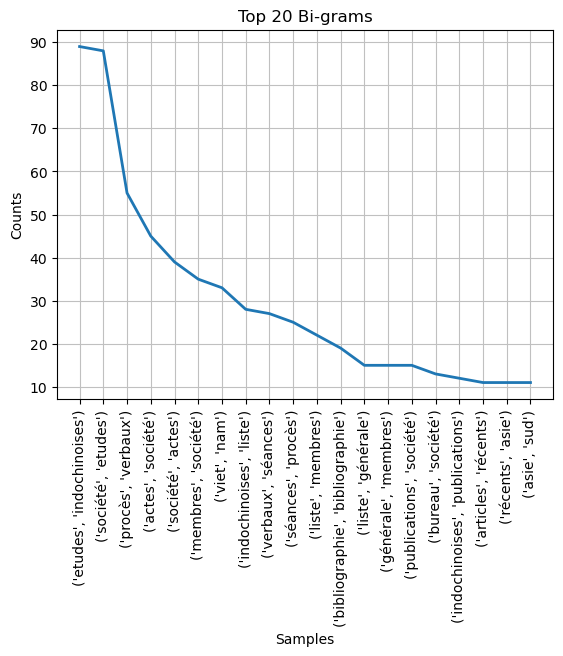
\includegraphics[width=12cm]{img/2.2.bigram-title.png}
    \caption{Bigram par titres}
    \label{fig:bigram-title}
\end{figure}

Un nuage de mots est une représentation visuelle de données textuelles qui est utilisée pour mettre en évidence les mots les plus fréquents dans un texte ou un corpus donné. C'est une technique de visualisation de données populaire qui offre un moyen rapide et intuitif de comprendre les termes ou les mots clés présents dans un ensemble de données.

\begin{figure}
    \centering
    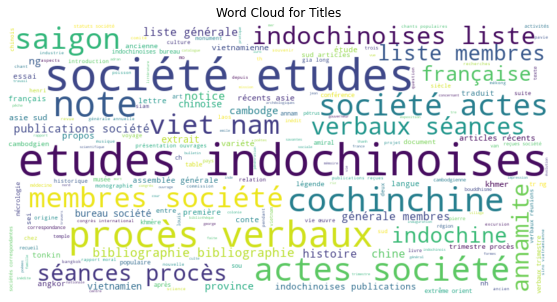
\includegraphics[width=12cm]{img/2.3.word_cloud_title.png}
    \caption{Nuage de mots par titres}
    \label{fig:nuage_titre}
\end{figure}

Le nuage de mots pour les titres est présenté dans la Figure \ref{fig:nuage_titre}, ce qui nous donne une idée des principaux sujets abordés dans le corpus. Comme pour les n-grams, cette visualisation nous permet de constater que les "études indochinoises" sont un thème récurrent dans l'ensemble des publications.

Un graphe de co-occurrence, également appelé réseau de cooccurrence ou matrice de cooccurrence, est un concept fondamental du NLP. Il est utilisé pour représenter et analyser les relations entre les éléments en fonction de leur cooccurrence dans un ensemble de données.

\begin{figure}[H]
    \centering
    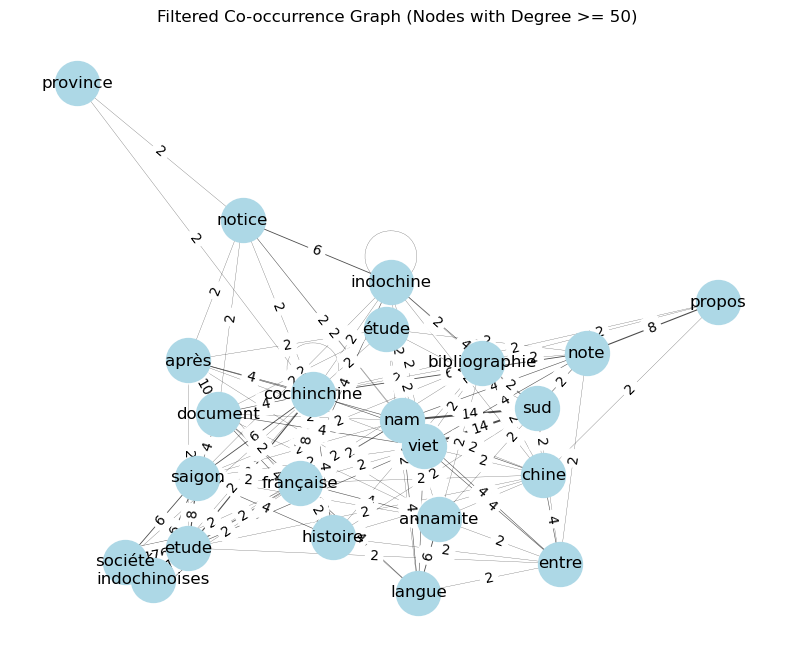
\includegraphics[width=12cm]{img/2.4.co-occurence-title.png}
    \caption{Graphe co-occurrence}
    \label{graph_cooc}
\end{figure}

Les mots qui co-apparaissent fréquemment sont susceptibles d'être sémantiquement liés, ce qui permet d'obtenir un aperçu de la structure sous-jacente du texte. Dans le cas de votre exemple avec les mots "étude", "société", et "indochinoise", on peut intuitivement constater que ces sujets sont liés à des termes tels que "Saigon", "français" et "histoire".


%%%%%%%%%%%%%%%%%%%%%%%%%%%%%%%%%%%%%%%%%%%%%%%%%%%%%%%%%%%%%%%%%%%%%%%%%%%%%%%%%%%%%%%%%%%%%%%%%%%%%%%%%%%%%%%%%%%%%%%%%%%%%%%%%%%%%%%%%%%%%%%%%%%%%%%%%%%%%%%%%%%%%%%%%%%%%%%%%%%%%%%%%%%%%%%%%%%%%%%%%%%%%%%%%%%%%%%%

\subsection{Exploration générale du corpus}
\subsubsection{Statistiques du Corpus}
Le tableau \ref{Tab:statscorpus} présente une description avec les statistiques simples de la taille du corpus.

\begin{table}[H]
\caption{Statistiques du corpus}
\centering
\bigskip
\begin{tabular}{lc}
    \hline
    Article &  916 \\
    Phrases &  474034  \\
    Mots &  6345322 \\
    \hline
\end{tabular}
 \label{Tab:statscorpus}
\end{table}
\bigskip

Les bigrammes et trigrammes du corpus sont visualisés dans la figure \ref{fig:bigram}. On y retrouve les collocations déjà rencontrées dans les titres, telles que "étude indochine", "procès verbal", "membre société", ainsi que des collocations plus spécifiques comme "extrême orient", "point vue", "phan thanh gian", etc.

\begin{figure}
\centering
\begin{subfigure}{0.6\textwidth}
    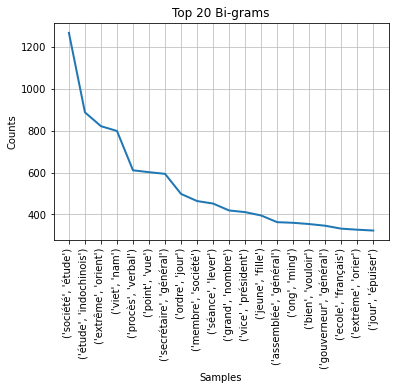
\includegraphics[width=\textwidth]{img/2.5.bigram.png}
    \caption{Bigrams}
    \label{fig:bigram}
\end{subfigure}
\hfill

\begin{subfigure}{0.6\textwidth}
    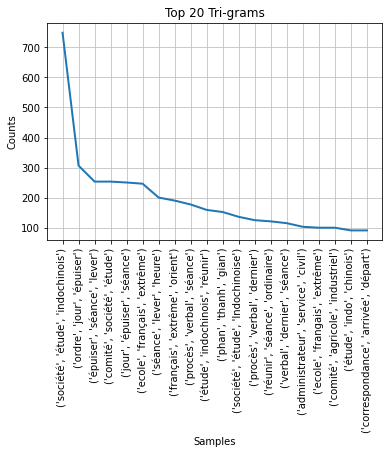
\includegraphics[width=\textwidth]{img/2.6.trigram.png}
    \caption{Trigrams}
    \label{fig:trigram}
\end{subfigure}
        
\caption{Collocations populaires du corpus}
\label{fig:ngrams}
\end{figure}
    
Dans la figure \ref{fig:nuage_corpus}, nous présentons un nuage de mots du corpus. Il est important de noter que les verbes les plus courants ont été exclus pour mettre en évidence les termes les plus intéressants :

\begin{figure}[H]
    \centering
    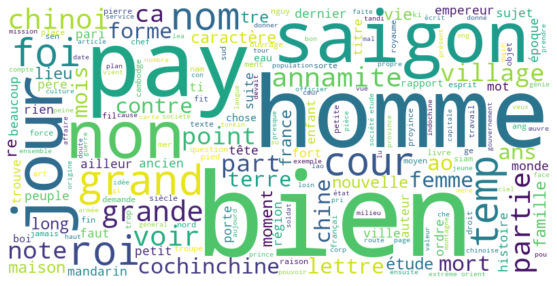
\includegraphics[width=12cm]{img/2.7.word_cloud_total.png}
    \caption{Nuages des mots du corpus}
    \label{fig:nuage_corpus}
\end{figure}

%%%%%%%%%%%%%%%%%%%%%%%%%%%%%%%%%%%%%%%%%%%%%%%%%%%%%%%%%%%%%%%%%%%%%%%%%%%%%%%%%%%%%%%%%%%%%%%%%%%%%%%%%%%%%%%%%%%%%%%%%%%%%%%%%%%%%%%%%%%%%%%%%%%%%%%%%%%%%%%%%%%%%%%%%%%%%%%%%%%%%%%%%%%%%%%%%%%%%%%%%%%%%%%%%%%%%%%%%%%%%%%%%%%%%%%%%%%%%%%%%%%%%%%%%%%%%%%%%%%%%%%%%%%%%%%%%%%%%%%%%%%%%%%%%%%%%%%%%%%%%%%%%%%%%%%%%%%%%%%%%%%%%%%%%%%%%%%%%%%%%%%%%%%%%%%%%%%%%%%%%%%%%%%%%%%%%%%%%%%%%%%%%%%%%%%%%%%%%%%%%%%%%%%%%%%%%%%%%%%%%%%%%%%%%%%%%%%%%%%%%%%%%%%%%%%%%%%%%%%%%%%%%%%%%%%%%%%%%%%%%%%%%%%%%%%%%%%%%%%%%%%%%%%%%%%%%%%%%%%%%%%%%%%%%%%%%%%%%%%%%%%%%%%%%%%%

\subsubsection{Suppression des mots vides}
La suppression des mots vides des données textuelles dans NLP offre plusieurs avantages, notamment la réduction du bruit, la réduction de la dimensionnalité et l'augmentation de la sensibilité aux termes importants. 
Un comptage a été mis en place pour estimer la proportion de mots vides dans le texte original, et il s'avère qu'ils représentent environ 4.12\% de l'ensemble du corpus.

Comparé à la liste des mots vides de NLTK, celle fournie par Spacy est plus complète, nous l'utilisons pour les analyses de modélisation de sujets qui nécessitent la suppression maximale des mots peu importants. Voici un exemple pour illustrer comment les mots vides sont supprimés en utilisant les listes de mots vides de Spacy et de NLTK :

\textbf{Texte original} : \textit{des liens sociaux des coutumes et des mœurs des religions et des philosophies qui commandent les cohésions et les poussées populaires étude des sciences et des littératures qui nourrissent intellectuellement les élites dirigeantes apparaissent de plus en plus nécessaires notre époque tous les peuples frémissent et ébranlent vers des destins nouveaux. Les débuts de étude systématique de extrême orient et le défrichement des sciences humaines d' asie ne datent que d'hier. et bon nombre des études faites commencent à peine à être diffusées. or la société des etudes indochinoises a le privilège plus rare dans le monde entier qu' on ne pense utiliser les concours de savants et de spécialistes qui ont une expérience directe des pays et des civilisations extrême}

\textbf{Texte traité par NLTK}: \textit{ lien social coutume mœur religion philosophie commander cohésion poussée populaire    étude science littérature nourrir intellectuellement élite dirigeant apparaître plus plus nécessaire    époque    tout peuple frémir    ébranlent vers destin nouveau début    étude systématique    extrême orient défrichement science humain    asie dater    hier bon nombre étude fait commencer    peine    être diffuser or société etude indochinoise avoir privilège plus rare monde entier penser    utiliser concours savant spécialiste avoir expérience direct pays civilisation extrême}

\textbf{Texte traité par Spacy} : \textit{ lien social coutume mœur religion philosophie commander cohésion poussée populaire    étude science littérature nourrir intellectuellement élite dirigeant apparaître nécessaire    époque    peuple frémir    ébranlent destin début    étude systématique    extrême orient défrichement science humain    asie dater    hier bon nombre étude commencer    peine    diffuser société etude indochinoise privilège rare monde entier penser    utiliser concours savant spécialiste expérience direct pays civilisation extrême.}
%%%%%%%%%%%%%%%%%%%%%%%%%%%%%%%%%%%%%%%%%%%%%%%%%%%%%%%%%%%%%%%%%%%%%%%%%%%%%%
\subsubsection{Analyse de sentiment}

Effectuez une analyse des sentiments pour évaluer le sentiment général ou les émotions exprimées dans le corpus de texte. J’utilise TextBlob un bibliothèque populaire dans ce domaine.

\textbf{Polarité:} La polarité fait référence au ton émotionnel ou au sentiment exprimé dans un morceau de texte. Il indique si le texte exprime un sentiment positif, négatif ou neutre.  La polarité est généralement mesurée sur une échelle numérique allant de -1 à 1, où  -1 représente un sentiment fortement négatif, 0 représente un sentiment neutre et 1 représente un sentiment fortement positif. Par exemple, un texte contenant des mots positifs comme « heureux », « amour » et « incroyable » aura un score de polarité positif. Un texte contenant des mots négatifs comme « triste », « haineux » et « décevant » aura un score de polarité négatif. Un texte contenant un mélange de mots positifs et négatifs peut avoir un score de polarité proche de 0, indiquant un sentiment neutre.

\begin{figure}[!ht]
    \centering
    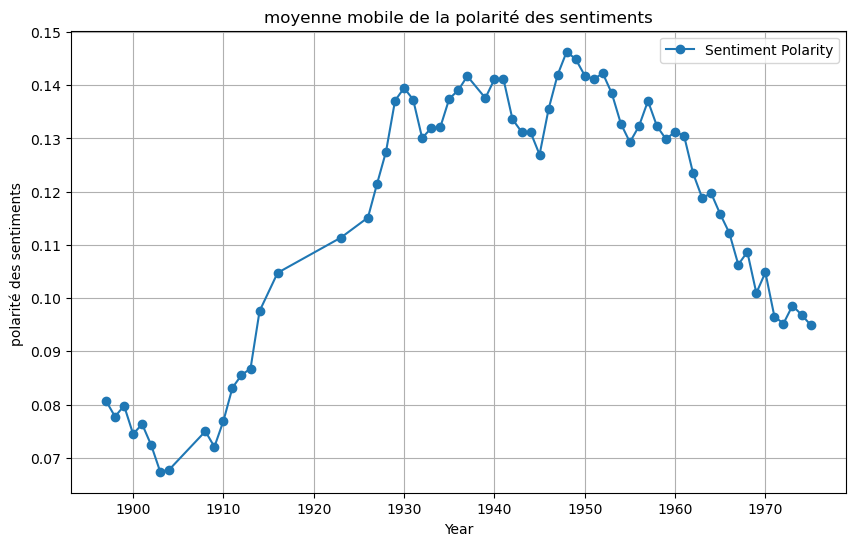
\includegraphics[width=12cm]{img/2.8.polarity_sentiment.png}
    \caption{Nuages des mots des titres}
    \label{fig:polar_senti}
\end{figure}

En général, les scores de polarité des documents sont assez faibles, variant entre 0.07 et 0.15, ce qui indique un sentiment plutôt neutre dans l'ensemble du corpus. Cela peut s'expliquer par le fait que les documents sont principalement des bulletins d'études, qui ont tendance à être informatifs et à contenir peu d'émotion. Cependant, on peut observer une augmentation continue de la polarité entre 1880 et 1940. Cette période a été témoin d'une influence coloniale importante en Indochine, principalement de la part des puissances coloniales françaises. Les sentiments exprimés dans le corpus peuvent refléter l'évolution des sentiments de la population locale, passant de la résistance initiale et du mécontentement sous le régime colonial à l'émergence des premiers mouvements nationalistes. Les sentiments pourraient devenir plus positifs à mesure que les gens commençaient à rechercher une plus grande autonomie. Ensuite, on observe la période pendant laquelle le gouvernement colonial français a commencé à se retirer d'Indochine, et en même temps, les nuances expressives des documents ont diminué pour atteindre un état plus neutre.

\textbf{Subjectivité} est la mesure dans laquelle un morceau de texte exprime un point de vue subjectif ou objectif. Cela indique à quel point le texte est basé sur des opinions, des sentiments ou des croyances personnelles plutôt que sur des faits ou des objectifs purement objectifs. La subjectivité est généralement mesurée sur une échelle numérique allant de 0 à 1, où 0 représente un texte très objectif ou factuel et 1 représente un texte hautement subjectif ou basé sur une opinion. Par exemple, un reportage objectif qui présente des faits et des chiffres sans opinions personnelles aura un faible score de subjectivité (proche de 0). Alors qu'un article de blog personnel ou une critique de produit exprimant des sentiments et des opinions personnels auront un score de subjectivité élevé (plus proche de 1).

Le changement de subjectivité des sentiments dans les documents de 1880 à 1975 peut être attribué à des facteurs historiques, politiques et socioculturels qui ont façonné le récit et les attitudes au fil du temps.

\begin{figure}[!ht]
    \centering
    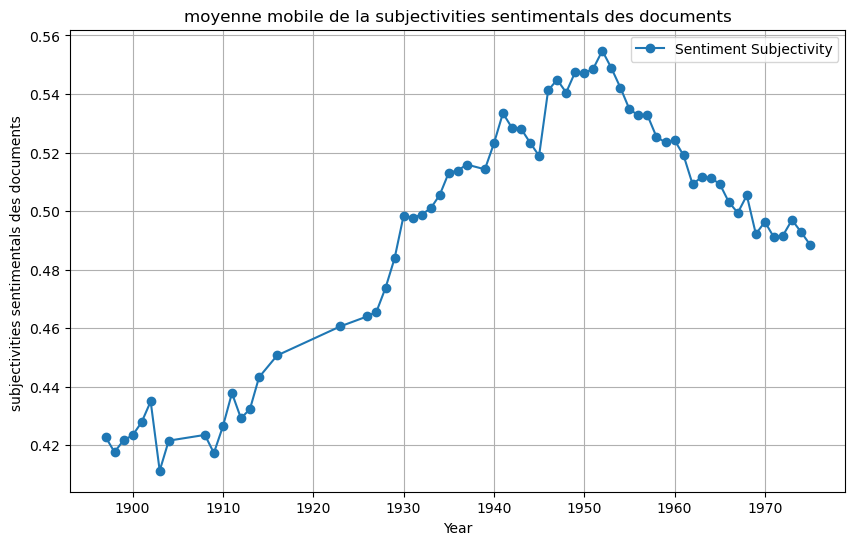
\includegraphics[width=12cm]{img/2.9.subjectivity_sentiment.png}
    \caption{Subjectivite sentimental}
    \label{fig:subject_senti}
\end{figure}

\textbf{Conclusion : }Analyser les sentiments au fil des années dans un corpus lié à l’Indochine peut être significatif pour les études historiques et culturelles. Cependant, elle doit être menée avec une orientation de recherche claire, en étant consciente des limites de l’analyse des sentiments et en tenant compte du contexte historique plus large. Les enseignements tirés d’une telle analyse peuvent contribuer à une meilleure compréhension de la façon dont l’Indochine a été perçue et représentée au fil du temps. 

 Les point de vue de Thomas Kuhn est "On  concevait  qu’en  ajoutant des résultats aux théories, on devrait se rapprocher toujours plus  du  vrai  au  fur  et  à  mesure  des  siècles.  Selon  Kuhn,  cela  ne  se  passe pas ainsi. Le progrès scientifique procède par une succession de périodes calmes et de ruptures. Pendant les périodes stables, la discipline se  développe,  organisée  autour  d’un  paradigme  dominant,  sorte  de  cadre théorique auquel adhère la communauté des professionnels du moment. Par exemple, la mécanique newtonienne a fonctionné ainsi du xviie siècle au début du xxe siècle sans être remise en cause. On y accumule des connaissances, mais aussi des problèmes à résoudre. Lorsque ces anomalies se multiplient, une crise survient, qui peut déboucher  sur  une  révolution  scientifique."\footnote{\cite{thomaskun08}}

 
\subsubsection{Analyse du vocabulaire des termes significatifs}

L'utilisation du terme "Annamite" jusqu'en 1948 dans la Figure \ref{fig:ananm_viet} reflète l'influence de la colonisation française sur la région et l'évolution politique et sociale qui a conduit à l'adoption du terme "Vietnamien" pour décrire le peuple et la nation du Vietnam. Les autorités coloniales françaises avaient une influence considérable sur la région et ont imposé leur propre terminologie et leur vision du monde aux habitants de la colonie. Le terme "Annamite" était historiquement utilisé pour désigner les habitants de la région qui correspond approximativement au nord et au centre du Vietnam moderne. Il provient du nom de l'ancien royaume d'Annam, qui existait avant la colonisation française. Les Français ont conservé ce terme pour désigner les Vietnamiens même après avoir élargi leur contrôle sur l'ensemble de l'Indochine. Le passage de l'utilisation du terme "Annamite" à "Vietnamien" en 1948 a coïncidé avec le déclin du colonialisme français en Indochine et le début du mouvement nationaliste vietnamien dirigé par Ho Chi Minh. Le changement de terminologie était également lié à la montée du nationalisme vietnamien et à l'affirmation de l'identité nationale vietnamienne distincte.

\begin{figure}[H] %[!ht]
    \centering
    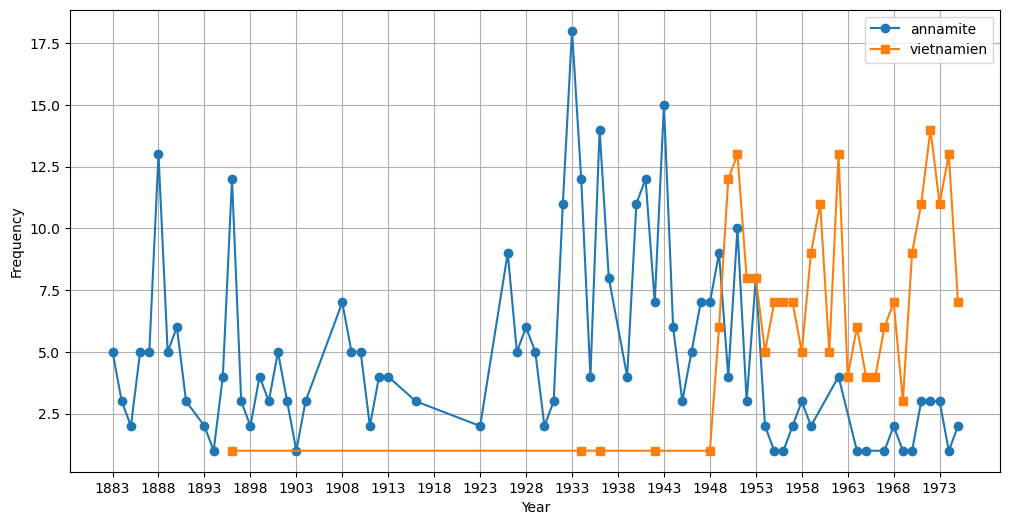
\includegraphics[width=12cm]{img/vietnam_annamite.png}
    \caption{Changement de fréquence d'utilisation entre les termes "annamite" et "vietnamien"}
    \label{fig:ananm_viet}
\end{figure}

On peut clairement observer un changement significatif dans la fréquence d'utilisation de ces deux termes dans la Figure \ref{fig:ananm_viet}. Tout d'abord, vers 1949, le terme "Vietnamien" émerge soudainement avec une utilisation plus répandue. Historiquement, en juillet 1949, le gouvernement provisoire de l'État du Vietnam a été établi, avec la nomination de Bao Dai en tant que chef de l'État. À partir de ce moment, le terme "vietnamien" a été rétabli officiellement. 

M. Cao-vân-Chiêu, ancien conseiller de l'Union Française lorsqu'il demanda, le 3 décembre 1953, à la tribune de l'assemblée versaillaise, que l'adjectif « vietnamien » fût substitué, dans tous les cas, à celui d'annamite qui réapparaissait parfois par inadvertance dans les textes officiels français. » 

Les deux termes, "vietnamien" et "annamite", représentent en réalité deux affirmations totalement différentes de l'identité nationale. Dans le contexte colonial, le terme "annamite" était souvent considéré comme péjoratif, même si, selon Jean Rispaud : 

« En tout cas, avant la deuxième guerre mondiale, les se nommaient eux-mêmes « gens d'Annam » et pas autrement, bien que ce nom sonnât désagréablement aux oreilles des lettrés qui en connaissaient l'origine. Tous les Occidentaux ont pu l'entendre comme moi en Indochine et d'innombrables témoignages écrits le confirment. »\footnote{\cite{vietnam}}

Un curieux problème historique : 
"An Nam" est un ancien nom du Vietnam, qui signifie "Sud Pacifié" et « qui avait été imposé par la Chine  en l'an 264 avant J.-C »\footnote{\cite{vietnam}}. à une époque où le pays était sous la domination du Nord. Ce nom avait pour intention de rappeler la vassalité du Vietnam envers la Chine, car le pays ne s'était pas rebellé ni n'avait fait la guerre. En revanche, le terme "Vietnam" (pays du Sud) affirmait l'indépendance du pays en tant qu'entité distincte, libre de toute colonisation.

Dans les années qui ont suivi, de 1933 à 1949, le terme "annamites" était largement utilisé dans la revue. Cela s'explique en partie par la période florissante du développement de la revue, caractérisée par un grand nombre de textes, ainsi que par la présence d'éminents intellectuels en tant qu'auteurs. Cette période a vu une augmentation des études sur le peuple vietnamien, ses coutumes et ses ethnies par rapport aux années précédentes.

Il est également intéressant de noter qu'à la dernière étape de l'élaboration du bulletin, de 1969 à 1975, le terme "annamites" a progressivement disparu au profit du terme "vietnamien". Cette évolution correspondait aux changements politiques de l'époque, où les Français n'avaient plus l'avantage. De plus, au sein du journal, de nombreux auteurs vietnamiens écrivaient sur leur propre pays et aspiraient à développer une identité nationale et scientifique pour le peuple vietnamien. Par exemple, certains articles d'auteurs vietnamiens en 1971-1972 reflétaient cette évolution.

\begin{itemize}
    \item L’expérience poétique et l’itinéraire spirituel de Han Mac Tu par Vo Long Te (1971)
    \item Quelques livres récents sur les études Vietnamien par Nguyen The Anh (1971)
    \item Nguyen Binh Khiem porte-parole de la sagesse populaire par Xuan Phuc (1971)
    \item Folklore du Sud du Vietnam : ong Hong, l’homme le plus riche de Nam Ky par Dao Van Hoi (1971)
    \item Dictionnaires vietnamiens par Vo Tong Le (1972)
    \item Nguyen Truong To, patriote réformiste, poète et homme d’action par Thai Van Kiem (1972)
    \item Enrichissement des forêts de conifères par introduction d’essences résineuses exotiques sur les Hautes Plateaux du Langbiang par Nguyen Van Thon (1972)
    \item Le culte de la Baleine par Thai Van Kiem (1972)
\end{itemize}

\begin{figure}[H] %[!ht]
    \centering
    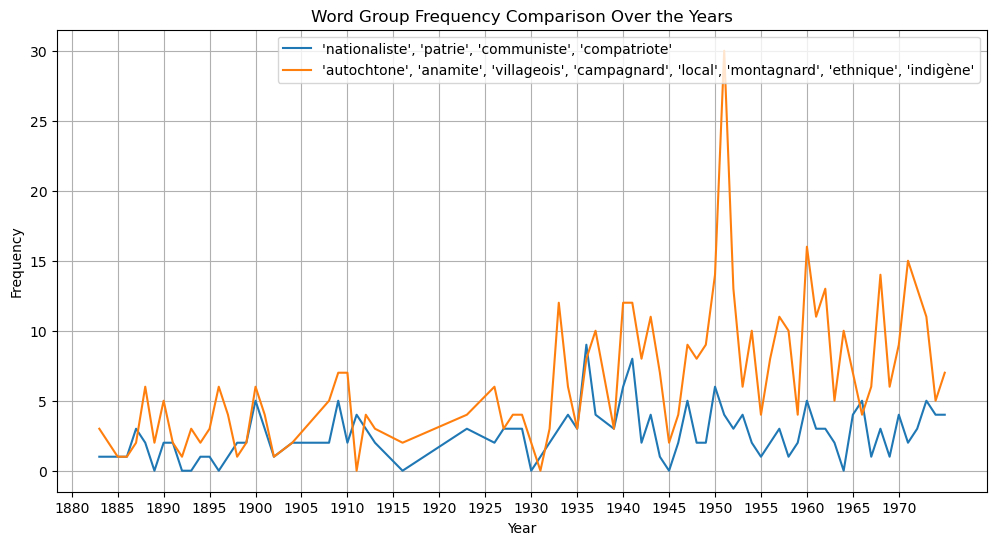
\includegraphics[width=12cm]{img/2.11.national_local.png}
    \caption{Évolution de la fréquence d'utilisation des termes "nationalisme" ou "localisme"}
    \label{fig:national_local}
\end{figure}
Nous portons également notre attention sur des sujets controversés afin de mesurer le niveau d'objectivité du corpus dans la figure \ref{fig:national_local}. Cependant, en ce qui concerne les thèmes liés au localisme, bien que les termes utilisés semblent parfois renvoyer à des minorités ethniques ou à des civilisations moins avancées, ils demeurent un élément récurrent dans l'ensemble du corpus. Les articles correspondants traitent souvent de questions d'ethnicité et d'ethnologie. De même, le nationalisme est abordé plus tard dans le corpus, mais la majorité des articles restent axés sur les études des pays indochinois et leurs aspects ethniques. La quantité accrue d'articles et l'expérience plus approfondie des auteurs entraînent également une augmentation du nombre de mots abordant ces sujets.

\begin{figure}[H] %[!ht]
    \centering
    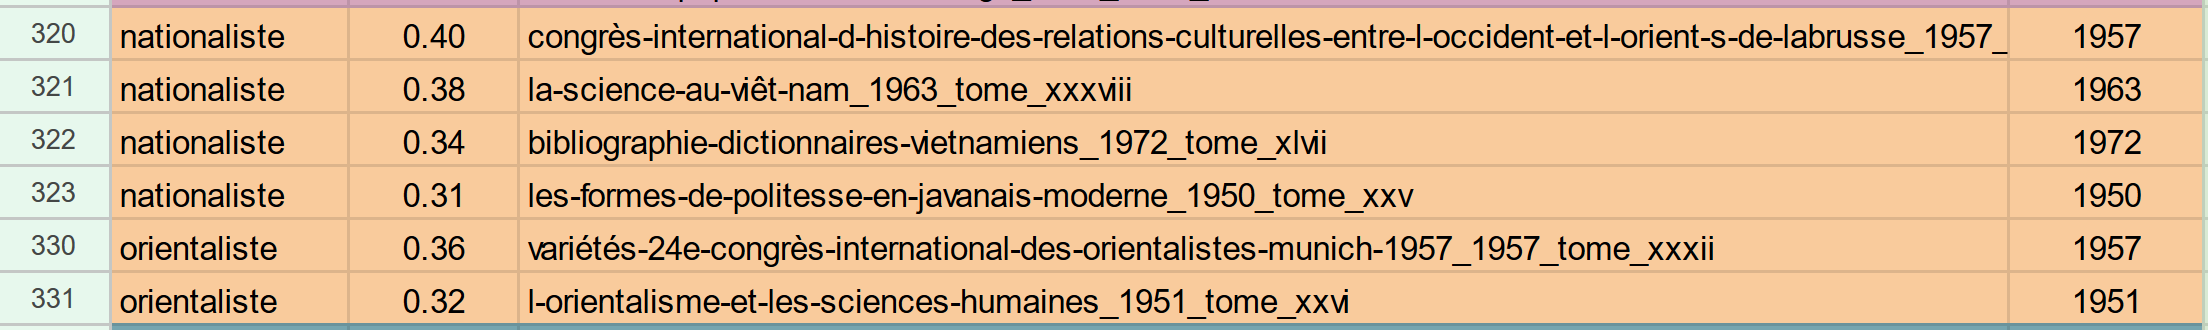
\includegraphics[width=1\linewidth]{img/nationaliste.PNG}
    \caption{Quelques exemples d'articles}
    \label{fig:enter-label}
\end{figure}

\begin{figure}[H] %[!ht]
    \centering
    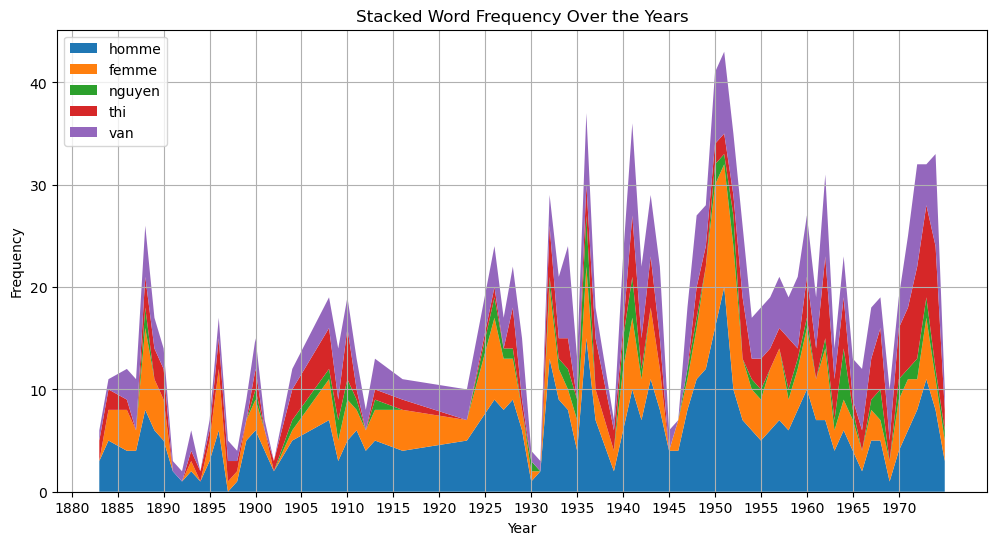
\includegraphics[width=12cm]{img/2.12.name_viet.png}
    \caption{Évolution de la fréquence d'utilisation des termes "homme", "femme" et des noms Vietnamiens}
    \label{fig:name_viet}
\end{figure}


Dans la Figure \ref{fig:mot_geo}, nous analysons l'utilisation de termes géographiques dans différentes régions de l'Indochine. Nous remarquons une répartition très équilibrée de la fréquence d'utilisation de ces termes, ce qui suggère que les publications du bulletin étaient équitablement réparties entre les différentes régions de l'Indochine à l'époque.

Le Tonkin et la Cochinchine étaient deux régions historiques situées dans l'ancienne Indochine française, en Asie du Sud-Est. 
Le Tonkin était situé au nord de l'actuel Vietnam.
Il était délimité approximativement par la rivière Rouge (Song Hong) au nord et par le 17e parallèle au sud, ce qui le séparait de la Cochinchine.
Le Tonkin comprenait les régions du delta du fleuve Rouge et des montagnes du Nord, et il était principalement peuplé par des Vietnamiens Kinh. Hanoï était la capitale du Tonkin.
La Cochinchine était située au sud de l'actuel Vietnam.
Elle était bordée par la mer de Chine méridionale à l'est, le Cambodge à l'ouest, et le Tonkin au nord. La Cochinchine était composée en grande partie de terres basses, y compris le delta du Mékong, et elle était connue pour sa fertilité. Sa principale ville était Saïgon, qui est aujourd'hui Ho Chi Minh-Ville.

\begin{figure}[H]
    \centering
    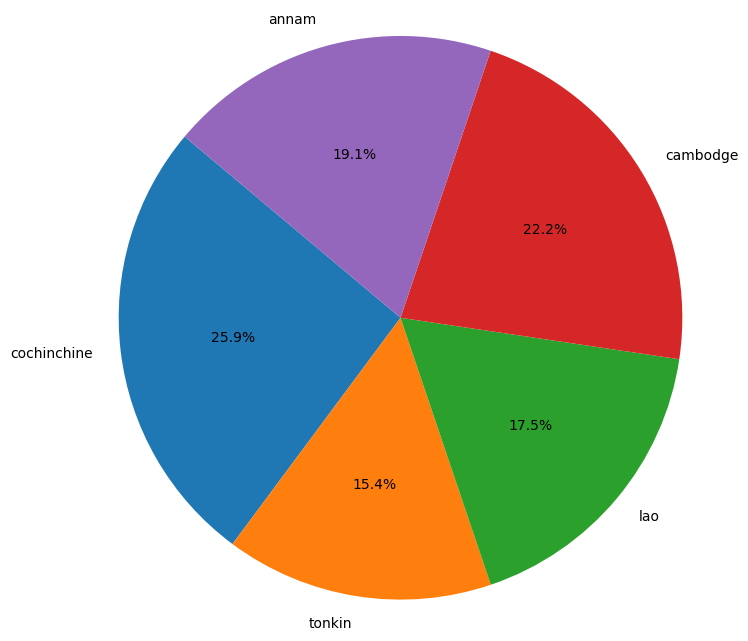
\includegraphics[width=12cm]{img/2.13.mot_geo.png}
    \caption{Répartition des termes des régions géographiques}
    \label{fig:mot_geo}
\end{figure}

Le Laos était l'une des composantes de l'Indochine française. Il était principalement considéré comme une région rurale et montagneuse, et son économie reposait sur l'agriculture, en particulier la culture du riz. Sous la domination française, le Laos a été intégré dans l'administration coloniale indochinoise, bien qu'il ait conservé une certaine autonomie locale. Pendant cette période, le Laos a été exposé à l'influence culturelle française, mais il est resté largement rural et peu développé sur le plan économique.

Le Cambodge, quant à lui, était une autre composante de l'Indochine française. Le Cambodge a une histoire riche et ancienne en tant que royaume khmer, mais il est devenu un protectorat français au XIXe siècle. Pendant la période coloniale, le Cambodge a été gouverné par une administration française, mais il a également conservé sa monarchie. Le Cambodge a connu une modernisation sous l'influence française, avec des développements urbains, l'introduction de l'éducation occidentale et des changements sociaux.

Effectivement, dans le corpus, les thèmes abordés ne sont pas répartis de manière égale selon les régions géographiques, mais chaque région a ses propres domaines d'intérêt distincts. Par exemple, au Vietnam, bien que les thèmes soient diversifiés, ils se concentrent souvent sur des sujets tels que la géographie, l'agriculture, la langue, etc. En revanche, le Cambodge présente des thèmes liés à la religion, à l'architecture et à la culture khmère, tandis que le Laos explore également sa culture ancienne, Le Tonkin avec la culture confucéenne et de riches éléments ethniques traditionnels, l'Annam est principalement axé sur les anciennes dynasties,etc.

Cependant, dans l'ensemble, le rapport entre les régions est assez équilibré, même si la Cochinchine, en tant qu'objet de recherche direct de la revue, compte naturellement un nombre plus important de contributions. Cette répartition reflète l'engagement de la revue à explorer et à documenter les aspects scientifiques, culturels et géographiques de chaque région de l'Indochine, contribuant ainsi à une compréhension globale de la région dans son ensemble.

Nous allons encore découvrir ces aspects historiques, culturels et économiques de ces régions dans les prochaines sections.
